% Template for PLoS
% Version 1.0 January 2009
%
% To compile to pdf, run:
% latex plos.template
% bibtex plos.template
% latex plos.template
% latex plos.template
% dvipdf plos.template

\documentclass[10pt]{article}

% amsmath package, useful for mathematical formulas
\usepackage{amsmath}
% amssymb package, useful for mathematical symbols
\usepackage{amssymb}

% graphicx package, useful for including eps and pdf graphics
% include graphics with the command \includegraphics
\usepackage{graphicx}

% cite package, to clean up citations in the main text. Do not remove.
\usepackage{cite}

\usepackage{color} 

% Use doublespacing - comment out for single spacing
%\usepackage{setspace} 
%\doublespacing


% Text layout
\topmargin 0.0cm
\oddsidemargin 0.5cm
\evensidemargin 0.5cm
\textwidth 16cm 
\textheight 21cm

% Bold the 'Figure #' in the caption and separate it with a period
% Captions will be left justified
\usepackage[labelfont=bf,labelsep=period,justification=raggedright]{caption}

% Use the PLoS provided bibtex style
%\bibliographystyle{plos2009}

% Remove brackets from numbering in List of References
\makeatletter
\renewcommand{\@biblabel}[1]{\quad#1.}
\makeatother


% Leave date blank
\date{}

\pagestyle{myheadings}
%% ** EDIT HERE **

\usepackage{pgfplots}
\usepackage{tikz}

%% ** EDIT HERE **
%% PLEASE INCLUDE ALL MACROS BELOW

%% END MACROS SECTION

\begin{document}

% Title must be 150 characters or less
\begin{flushleft}
{\Large
\textbf{Digital language death revisited}
}
% Insert Author names, affiliations and corresponding author email.
\\
Martin Juh\'asz and Andr\'as Kornai %
\\
%\bf{1}
Institute of Mathematics, Budapest University of Technology and Economics\\
%Computer and Automation Research Institute, Hungarian Academy of Sciences, Budapest, Hungary\\
%\\Department of Computer Science, Boston University, Boston MA\\
$\ast$ E-mail: juhaszm1@edu.bme.hu, kornai@math.bme.hu
\end{flushleft}

% Please keep the abstract between 250 and 300 words
\section*{Abstract}

In the earlier \cite{Kornai:2013c} we argued that 
Of the approximately 7,000 languages spoken today, some 2,500 are generally
considered endangered. Here we argue that this consensus figure vastly
underestimates the danger of digital language death, in that less than 5\% of
all languages can {\color{black} still ascend to the digital realm}. We present evidence of a
massive die-off caused by the digital divide.

%\section*{Author Summary}

\section*{Introduction}

The biological metaphor of viewing languages as long-lived organisms
goes back at least to Herder \cite{Morpurgo-Davies:1992},  and has been 
%(see Morpurgo-Davies 1992: 84),
clearly stated in {\it The Descent of Man} \cite{Darwin:1871}:
%(Darwin 1871: 67)

\begin{quote}

The formation of different languages and of distinct species, and
the proofs that both have been developed through a gradual process,
are curiously parallel. (...) We find in
distinct languages striking homologies due to community of descent,
and analogies due to a similar process of formation. The manner in
which certain letters or sounds change when others change is very like
correlated growth. (...) Languages, like organic beings, can
be classed in groups under groups; and they can be classed either
naturally according to descent, or artificially by other characters.
Dominant languages and dialects spread widely, and lead to the gradual
extinction of other tongues. 

\end{quote} 
 
While not without its detractors \cite{Frank:2008}, the
%(see e.g. Frank 2008), the 
biological metaphor has been widely accepted both in research concerning 
language death \cite{Nettle:2000},\cite{Crystal:2002} and in 
%(Nettle and Romaine 2000, Crystal 2000) 
guiding political action (see e.g. the United Nations Environment Programme
Convention on Biological Diversity,\cite{UN_biodiv:2004}). {\color{black}
% UNEP/CBD/AHTEG-2010-Ind/1/INF/7),
Here we investigate the phenomenon of {\it digital ascent} whereby languages
enter the space of digitally mediated communication. We could 
extend the metaphor and talk about the digital {\it hatching,
  pupation,} or {\it metamorphosis} of languages, but would gain little 
by doing so, since we can only speculate about further,
post-digital stages in the life cycle of languages. 
%The main finding of 
%our study is the statistically overwhelming failure to ascend that is our main finding would
%have to be discussed in the emotionally charged language of stillbirth,
%abortion, or arrested development. 

In this paper, we bring the traditional methods of language vitality
assessment to the digital realm. First we transfer the criteria themselves:
instead of speaker population we look at the online population, instead of
vigorous oral use we look at vigorous online use, and so forth, see Background
(i)-(v). Second, we collect data from online sources that reveal the relevant
variables or at least provide acceptable proxies for these, see
Materials. Third, we introduce a four-way classification into digitally
thriving (T), vital (V), heritage (H), and still (S) languages, roughly
corresponding to the amount of digital communication that takes place in the
language, and manually select prototypical seeds for these classes, see
Methods. Finally, multinomial logistic classifiers are built on the seeds and
are applied to the rest of the data, see Results.  This four-stage method is
shown to be robust, and remarkably independent of the manual choice of seeds,
see Discussion. The Conclusions section interprets our main result, that the
vast majority of the language population, over 8,000 languages, are digitally
still, that is, no longer capable of digital ascent.

\section*{Background}
}
%and we adopt it without much further discussion, together with the 
%standard time horizon of one hundred years used in most studies.

A language may not be completely dead until the death of its last speaker, but
there are three clear signs of imminent death observable well in advance.
First, there is {\it loss of function,} seen whenever other languages take
over entire functional areas such as commerce. Next, there is {\it loss of
  prestige}, especially clearly reflected in the attitudes of the younger
generation. Finally, there is {\it loss of competence}, manifested by the
emergence of `semi-speakers' who still understand the older generation, but
adopt a drastically simplified (reanalyzed) version of the grammar.  The
phenomenon has been extensively documented e.g. in Menomini \cite{Bloomfield:1927},
%(Bloomfield 1927),
Gaelic \cite{Dorian:1981},
%(Dorian 1981), 
and Dyrbal \cite{Schmidt:1985}.
%(Schmidt 1985).

In the digital age, these signs of incipient language death take on the
following characteristics. Loss of function {\it performed digitally}
increasingly touches every functional area from day to day communication
(texting, email) to commerce, official business, and so on.  Loss of prestige
is clearly seen in the adage {\it If it's not on the web, it does not exist},
and loss of competence boils down to the ability of raising digital natives
\cite{Prensky:2001} in your own language. {\color{black} Digital ascent is the
  opposite process, whereby a language increasingly acquires digital functions
  and prestige as its speakers increasingly acquire digital skills.} 

%A language that survives in the traditional sense may at the same time die a
%digital death, we will discuss several examples as we go along.

Language endangerment and language death, in the traditional sense, are widely
investigated and actively combated phenomena. The modern EGIDS classification
\cite{Lewis:2010} extends the Graded Intergenerational Disruption Scale
(GIDS) of Fishman \cite{Fishman:1991} to the following 13 categories: 0. International;
1. National; 2~Provincial; 3 Wider communication; 4 Educational; 5 Developing;
6a Vigorous; 6b Threatened; 7 Shifting; 8a Moribund; 8b Nearly Extinct; 9
Dormant; 10 Extinct. Categories 7-8b are considered endangered in the UNESCO
Atlas of the World's Languages in Danger \cite{Mosley:2010}, and categories 9-10 are
considered extinct. Since these comprise only 17\% of the world's languages,
with another 20\% (category 6b) vulnerable, one may get the impression that
the remaining 63\% (these numbers are from \cite{Simons:2013}) of the
%Simons  and Lewis 2013) 
world's languages are more or less in good shape. While this may be true in
the traditional sense, the main finding of our paper will be that the
{\color{black} vast majority (over 95\%) of languages have already lost the
  capacity to ascend digitally.}

Since digital(ized) data persists long after the last speaker is gone, we
cannot simply equate {\color{black} failure to ascend} with lack of online
data. We will make a distinction between digital {\it heritage} status, where
material is available for research and documentation purposes, but the
language is not used by native speakers (L1) for communication in the digital
world, and digitally {\it {\color{black} still}} status, characterized by lack
of even foreign user (L2) digital presence. It is of course very important to
move languages from the {\color{black} still} to the heritage stage, and there
are significant efforts under way to bring data and metadata about languages
online and to make both lexical resources and primary texts web-accessible,
see the Materials section for an introduction to these.  In the Results
section we will see that such efforts, laudable as they are, actually
contribute very little to the digital vitality of endangered languages.  Just
as the dodo is no less extinct for skeleta, drawings, or fossils being
preserved in museums of natural history, online audio files of an elder
tribesman reciting folk poetry will not {\color{black} facilitate digital
  ascent, and both still and heritage languages are digitally dead in the
  obvious sense of not serving the communication needs of a language
  community.}


%This is a considerably higher bar than having 
%digital(ized) material available in a language: for example 

%Some of
%these, such as Ikorom, see {\tt
%  http://www.endangeredlanguages.com/lang/ibe-iko}, have no ISO 639 code yet.

{\color{black} Digital ascent is a relatively new phenomenon,} especially on
the hundred year timescale common in studies of language death.  Digital
communication was not an important arena of language functionality until the
spread of electronic document creation in the 1970s; the internet and email in
the 1980s; the web and blogging in the 1990s; wikis and text messaging (SMS)
in the 2000s. Our approach will nonetheless be conservative inasmuch as we
simply adopt the standard conceptual framework, and the standard yardsticks,
to the digital domain. We will also try to be maximally conservative in the
sense that we will interpret the evidence favorably wherever we can, so as to
minimize false alarms.  There are five confluent factors we consider: (i) the
size and demographic composition of the language community; (ii) the prestige
of the language; (iii) the identity function of the language; (iv) the level
of software support; and (v) wikipedia. The last two may superficially look
peculiar to the digital domain, but as we shall see, they are just convenient
proxies for assessing a traditional yardstick, the functional spread of the
language.

\bigskip
(i) {\it Community size.} The primary traditional measure of vitality is the
size and generational composition of the language community. In the digital
realm, what we are interested in is the number of digital natives in the
language. Since the phenomenon is new, the demographics are highly favorable:
once the language community starts creating content by sending text messages,
writing blogs, and building wikis, we can reasonably expect that the younger
generation will follow suit, especially as digital fora like Facebook are
increasingly becoming a means for parents and grandparents to stay in touch
with their children. Therefore, we need to assess only the size of the wired
community separately, and can assume its demographic composition to be
uniformly good.

State censuses generally address the question of linguistic and national
identity, and tribe sizes are well known within the community, so it is
generally not hard to get at least a rough order of magnitude estimate on the
number of speakers. However, in and of itself a large and sustainable
population cannot guarantee digital ascent -- what we need to
consider is population {\it actively engaged in digitally mediated
  interaction}. Passive consumption of digital material, especially digital
material in an encroaching language, is irrelevant, if not actively harmful to
the survival of a threatened language. Michael Krauss' famous remark
``Television is a cultural nerve gas...odorless, painless, tasteless. And
deadly.'' \cite{Cazden:2003} applies to the web just as well.
%(Cazden 2003)

Since neither the size of the digitally enabled population nor the digital
suitability/prestige of the language are measured by censuses or other regular
surveys, we must resort to proxies in assessing digital vitality. The real
issue is {\it the amount of digitally mediated communication that takes place}
in the language. Ideally, we should capture all videoconference (Skype),
cellphone, Twitter, Facebook, etc. communication and measure the proportion of
material in the language in question.  Modern language technology has already
solved the problem of language identification, the Cr\'ubad\'an Project \cite{Scannell:2007}
actually builds such software for each language. As this technology in no way
relies on understanding the contents, privacy concerns are minimized and the
barriers to the direct measurement of digital language vitality are primarily
organizational: we need to put safeguards in place to make sure that the data
will be anonymized, that the people whose communications are monitored give
their permission, and so forth. Until such a comprehensive study is conducted,
we must use {\it the publicly available textual material} as our proxy -- this
has the advantage that all such material was put there knowingly by their
authors, so concerns of privacy are resolved in advance. The size of online
holdings (excluding wikipedia, see (v) below) was assessed by web
crawling. Our methods are described in \cite{Zseder:2012}, and some of the
results are made available for public download at {\tt
  http://hlt.sztaki.hu/resources/webcorpora.html}.

\bigskip
(ii) {\it Prestige.} The second most important measure of vitality is
prestige. Since digital communication is universally viewed as more
prestigious than communication by traditional means, the intergenerational
disruption actually acts in favor of digital {\color{black} ascent}, provided the new
generation has both the digital means and the interest in language use. In
digitally vital languages this happens quite effortlessly and automatically,
but languages the new generation no longer considers cool are caught in a
pincer movement, with the old generation unable and unwilling to enter the
digital world and the younger generation no longer considering the old
language relevant. They may not be semi-speakers in the technical sense, as
they retain full control over the grammar and vocabulary, but at the same time
they may consider the language inappropriate for dealing with the digital
realm. An almost laboratory pure example is provided by the two officially
recognized varieties of Norwegian, Bokm\aa l and Nynorsk. For many years, the
two wikipedias were of roughly equal size, and the best estimates \cite{Rehm:2012}
%(De Smedt et al 2012) 
put the proportion of language users at 7:1. By now, the Bokm\aa l wikipedia
is four times the size of the Nynorsk wikipedia, but Nynorsk is still in the
top 50. With a sizeable population of speakers that enjoy a high standard of
living, a nearly saturated personal computer market, and good access to
broadband networks, based solely on census data and wikipedia statistics
Nynorsk would appear a prime candidate for {\color{black} digital ascent}.  Yet
crawling the {\tt .no} domain demonstrates a striking disparity: we could find
1,620m words {\color{black} (tokens)} of Bokm\aa l but only 26m words in
Nynorsk. Considering that official (government and local government) pages are
published in both varieties, the actual proportion of user-generated Nynorsk
content is well under 1\%. In spite of a finely balanced official language
policy propping up Nynorsk, the Norwegian population has already voted with
their blogs and tweets to take only Bokm\aa l with them to the digital age.

The same phenomenon can be seen at the other side of the digital divide.  As
an example consider Mandinka, {\color{black} which is, besides Swahili,}
perhaps the single best known African language for the larger American
audience, thanks to Alex Hailey's {\it Roots}. With 1.35m speakers, and
official status in two countries (Senegal and The Gambia), Mandinka is neither
endangered nor threatened in the traditional sense -- SIL puts its EGIDS
rating at 5 (developing) and notes the positive attitude speakers of all ages
have toward the language.  However, its {\color{black} failure to digitally
  ascend} appears a foregone conclusion: literacy in the language is below
1\%, and the wikipedia incubator \cite{MandIncu}
has not attracted a single native speaker.


\bigskip
(iii) {\it Identity function.} As we will primarily rely on written material,
particular care needs to be taken to distinguish {\it passive} (read only) web
presence such as lexicons, classical literature, or news services, from {\it
  active} use in a broad variety of two-way contexts such as social networks,
business/commerce, live literature, etc. Language is for communication, and
passive presence indicates only efforts at preservation, often by scholars
actually outside the language community, not digital vitality. As an example
consider Classical Chinese, a language with a sizeable wikipedia, nearly 3,000
articles, and a remarkable user community of over 30,000 L2 users. There are
also significant text holdings elsewhere (see in particular {\tt
  http://ctext.org}). At the same time, the top-level question in
\cite{Lewis:2010}, which probes the identity function of a language clearly
puts Classical Chinese in the Historical/Heritage category, {\color{black} there defined as 
follows}: 

\medskip
\begin{quote}
{\it Historical} The language has no remaining speakers and no community which
associates itself with the language as a language of identity. There are no
remaining functions assigned to the language by any group (...)\\
{\it Heritage} There are
no remaining L1 speakers, but there may be some emerging L2 speakers or the
language may be used for symbolic and ceremonial purposes only. 
\end{quote}

%Joshua Fishman (1991) Reversing Language Shift: Theory and Practice of
%Assistance to Threatened Languages. Clevedon : Multilingual Matters. 

%Assessing endangerment: Expanding Fishman's GIDS M. Paul Lewis and Gary
%F. Simons. Revue Roumaine de Linguistique 55(2):103-120


\bigskip

(iv) {\it Functional domains.} Initially, digital word processing was restricted to
large organizations and printing presses, but with the spread of PCs, desktop
publishing became available at the household level. Similarly, the function of
making public announcements, until recently restricted to the village worthy,
became available to individuals, who can post on bulletin boards or
(micro)blog. Altogether, the digital age ushered in, or made more accessible,
many forms of communication hitherto restricted to small elites, and this is
undoubtedly one of its main attractions. But for a language to spread to these
new or newly democratized functional areas, one generally needs a bit of
software. (The main exception is cellphone usage, which we had to ignore in
this study for lack of data.) To quantify software support we use a simple
three-stage hierarchy, roughly analogous to the questions probing literacy 
status in EGIDS{\color{black}, see the Methods section}.

\medskip
(v) {\it Wikipedia.} Since digital {\color{black} ascent} means active use of the language
in the digital realm, we need to identify {\it at least one} active online community
that relies on the language as its primary means of communication. There may
be small bulletin boards, mailing lists, Yahoo, or Google groups scattered
around, but experience shows that Wikipedia is always among the very first
active digital language communities, and can be safely used as an early
indicator of some language actually crossing the digital divide. The reason is
that children, as soon as they start using computers for anything beyond
gaming, become aware of Wikipedia, which offers a highly supportive
environment of like-minded users, and lets everyone pursue a goal, summarizing
human knowledge, that many find not just attractive, but in fact instrumental
for establishing their language and culture in the digital realm. To summarize
a key result of this study in advance: {\it No wikipedia, no {\color{black} ascent}.}

The need for creating a wikipedia is quite keenly felt in all digitally
{\color{black} ascending} languages. This is clearly demonstrated by the fact that currently
there are 533 proposals in incubator stage, more than twice the number of
actual wikipedias.  In fact, the desire to get a working wikipedia off the
ground is so strong as to incite efforts at gaming the ranking system used by
wikipedia, which sorts the various language editions at {\tt
  http://meta.wikimedia.org/wiki/List\_of\_Wikipedias} simply by number of
articles. The most blatant of these Potemkin wikipedias is \#37, Volap\"{u}k,
which is based almost entirely on machine-generated geographic entries such as
{\sc Kitsemetsa} {\it Kitsemetsa binon vilag in graf\"an: L\"a\"ane-Viru, in
  Lestiy\"an. Kitsemetsa topon videt\"u 58$^0$55' N e lunet\"u 26$^0$19' L.}
{\color{black} `Kitsemetsa is a village in L\"a\"ane-Viru County, in Estonia. It
  is at at latitude 58$^0$55' N and longitude 26$^0$19' E.' The Methods
  section discusses how  the effects of   such gaming can be removed.}

\section*{Materials}

All our data come from public repositories accessed between June 2012 and
March 2013. A consolidated version of our main data table, 8,426 rows by 92
columns, is available as Data Supplement 1. {\color{black} Here we provide only
  a brief overview of the main data sources, see the Appendix for further
  details. The data is intended to cover the entire population of the world's
  languages -- some lacunae may remain, but internal consistency checks
  suggest that our coverage is over 95\%.}

The primary registry of data about the world's languages, now charged with
maintaining the ISO 639 standard for language codes, is the Ethnologue
database of the Summer Institute of Linguistics (SIL International), see {\tt
  http://www.ethnologue.com}. The latest (2012/02/28) publicly available
version of the database distinguishes 7,776 languages, among them 376 that
died since 1950 when SIL started to maintain the list.

We consulted several other sources, and our own dataset is larger by about
10\% for the following reasons. First, we didn't discard ancient/reconstructed
languages such as Classical Chinese or Proto-Indo-European and
artificial/constructed languages like Peano's Interlingua (Latin Sine
Flexione), which are by design out of scope for the Ethnologue. Second, our
sources cover several languages that have only been recently discovered and
have not yet completed the registry process: an example would be Bagata, a
language spoken by one of the Scheduled Tribes in Andhra Pradesh. Third, we
considered language groupings with online activity like Akan and Bihari
irrespective of whether they meet the SIL criteria for `macrolanguage'.
Whenever we encountered languages with no ISO code, and no code on the
Linguist List (see {\tt http://linguistlist.org}), we generated a
non-authoritative internal code that begins with {\tt xx} so as to maintain
unique identifiers suitable for joining rows from different sources. For less
commonly taught languages, we generally mention the ISO code (three lowercase
letters) because the language names themselves are often subject to
considerable spelling variation.  Altogether, we have 7,879 ISO codes (the
number is larger than the size of the February 2012 dump because the site now
provides codes for many newly registered languages), with the balance coming
from other sources, to which we now turn.

Perhaps the best organized of these is the Open Language Archives Community,
`an international partnership of institutions and individuals who are creating
a worldwide virtual library of language resources', see {\tt
  http://www.language-archives.org}. OLAC has some data for 7,478 of the 7,776
languages with ISO codes.  Neither OLAC nor Wikipedia will consider languages
without ISO code, so the lack of ISO status could in principle be a handicap
{\color{black} for digital ascent}. In practice, however, our conclusions can
only be strengthened by the inclusion of these unregistered languages since
they are already at the margin, with EGIDS level 6b or worse, while
{\color{black} failure to ascend} affects many languages at EGIDS level 4 or
even better.

The last source aiming at encyclopedic completeness is the Endangered
Languages Project hosted at {\tt http://www.endangeredlanguages.com} which consolidates
data from the Catalogue of Endangered Languages (ELCat), produced by the
University of Hawai'i at Manoa, and The Institute for Language Information and
Technology (The Linguist List) at Eastern Michigan University. We accessed the
database on 2013/03/15, when it contained data for 3,175 languages. ELP uses 
a different scale of vitality, with categories critically endangered; 
severely endangered; endangered; threatened; and vulnerable, which correlate 
well with the higher EGIDS categories but are independently assessed. Since 
ELP considers vital languages (which are generally EGIDS 6a or less) out of 
scope, the fact that a language has no ELP page is generally a good sign. with 

Less encyclopedic, but very relevant to our purposes, is the website of the
Cr\'ubad\'an Project, see {\tt
  http://borel.slu.edu/crubadan}, which collects language data for endangered
languages on the web. Version 2 covered 1,322 languages 2013/03/15 when we
accessed the data, Version 1 started with 1,003 in 2006.  The Cr\'ubad\'an
Project, quite independent from us, but consistent with our methodology, chose
not to harvest material from closed archives such as the Rosetta Project (see
{\tt http://rosettaproject.org}) or metainformation such as the grammatical
features collected in The World Atlas of Language Structures (see {\tt
  http://wals.info}), since these are in no way indicative of digital use by
native speakers.

Another highly relevant website is Omniglot, `the online encyclopedia of
writing systems and languages', see {\tt http://www.omniglot.com}. Literacy in
the traditional sense is a clear prerequisite of digital literacy, and
languages without mature writing systems are unlikely to {\color{black}
  digitally ascend}.  Note that there are only 696 languages listed in
Omniglot, and many of these are ancient or constructed languages without a
live community.  Even more relevant to our purposes is the level of support
for computer-mediated activity in a given language. Here our basic data comes
from inspecting Microsoft and Apple products for two levels of language
support: {\it input} and {\it OS}. Input-level support means the availability
of some specific method, such as Kotoeri for Japanese, to enter text in the
writing system used for the language. Without an input method, digital
{\color{black} ascent is impossible,} but the converse unfortunately does not
hold: the existence of some input method by no means guarantees an easy way to
create text in the language, let alone vigorous digital language use. OS-level
support means that all interaction conveyed by the operating system, such as
text in dropdown menus or error messages, are provided in the language in
question.

There are many languages with standard input methods but no standardized
orthography, and the next step up the digital ladder is a spellchecker. The
Cr\'ubad\'an Project also considers this a relevant factor, and lists
explicitly whether a Free/Libre Open Source Software (FLOSS) spellchecker
exists. We also looked at {\tt HunSpell} (the largest family of FLOSS
spellcheckers, see \cite{Nemeth:2004}) for each language, and assessed its
coverage by computing the percentage of words it recognizes in the wikipedia
dump. Any number below 50\% indicates the spellchecker is not mature.

Standardized orthography enables not just collective works like Wikipedia,
itself an important indicator of digital vitality, but also the creation of
larger documents. Again, the Cr\'ubad\'an Project considers this a relevant
factor, and lists whether the Bible and the Universal Declaration of Human
Rights (UDHR) are available online. Collecting larger corpora, the lifeblood
of modern language technology efforts, also requires standardized spelling.
The relationship of digital language vitality and more sophisticated tools of
modern computational linguistics such as parsers, speech and optical character
recognition software, information extraction, and machine translation tools
will be discussed in the next section. 

\section*{Methods}

{\color{black} The EGIDS scale already comes with a clear notion of ascent,
  from oral use only (category 6) to acquiring literacy (5) and `vigorous oral
  use (...) reinforced by sustainable literacy' (4). Further steps up the
  traditional scale are predicated on the level of (official) use: `used in work
  and mass media without official status to transcend language differences
  across a region' (3); `used in education, work, mass media, and government
  within officially recognized regions of a nation' (2); `used in education,
  work, mass media, and government at the nationwide level' (1); and
  `widely used between nations in trade, knowledge exchange, and international
  policy' (0) \cite{Quakenbush:2012}. In the digital realm, it is also
  literacy that provides the pivotal step, and we begin by describing the main
  stages of acquiring it.}

Stage one is some kind of {\it locale} or {\it i18n} (computer shorthand for
`internationalization') support that enables the input (writing) and output
(reading) of native characters. On the whole the Unicode standard, already
covering more than a hundred scripts and with a well-established mechanism for
adding new ones, provides a solid basis for bringing any language to the
digital age, as long as it is written (signed languages will be discussed
separately). When a language is listed in Omniglot, we can assume it is past
stage one. A weaker condition is the availability of online text in OLAC, a
stronger condition would be the availability of an input method.

For the second stage we need a variety of word-level tools such as
dictionaries, stemmers, and spellcheckers. Here support is more spotty -- even
the most broadly used tool, HunSpell \cite{Nemeth:2004}, is available only for
129 languages, {\tt http://hlt.sztaki.hu/resources/hunspell}. In spite of the
uneven coverage and quality of these tools, they already represent a level of
maturity that is very hard to match by an underresourced language. This is
because spellcheckers enforce the unified literary standard of a koin\'e, with
significant suppression of individual and dialectal variation. This stage was
reached by English only in the 15th century (primarily as a result of the
efforts of William Caxton), and many of the languages discussed here have
neither undergone the painful process of koin\'e formation driven by internal
needs nor want it to be imposed on them externally \cite{smh:2006}. 

The third stage requires phrase- and sentence-level tools that can only be
built on some preexisting character- and word-level standard, such as
part-of-speech taggers, named entity recognizers, chunkers, speech
recognition, and machine translation. In the tables presented at {\tt
  http://www.meta-net.eu/
  whitepapers/key-results-and-cross-language-comparison} not even English has
`Excellent' support in these higher areas, which are key to avoiding long-term
function loss. We surveyed Google Translate to probe this increasingly
important area of functionality, but we emphasize here that stage three has
more to do with the line between our top two categories, thriving (T) and
vital (V), while our primary concern is with the gap between
vital and {\color{black} still (S) languages}. We have not surveyed speech and character recognition
software, not because they are any less important, but because their quality
still improves at a fast pace, and languages that lack these today may well
acquire them in a hundred years.

{\color{black} Let us now describe the resolution of the classification system proposed
here. In contrast to the 8 categories used in GIDS and the 13 used in EGIDS,
we will identify only four classes of languages we call digitally {\bf
  T}hriving, {\bf V}ital, {\bf H}eritage, and {\bf S}till, roughly
corresponding to the volume of active language use in the digital
realm. Accordingly, the decision tree presented in Fig.~1 of \cite{Lewis:2010}
will be drastically simplified: we will have a major decision, whether a
language is actively used in the digital realm, and two supplementary
distinctions. The primary goal of our work is to investigate the dead/alive
distinction in the digital domain, with the finer distinctions between degrees
of ascent (vital versus thriving) and degrees of death (still versus
heritage) seen as secondary.}

One possible method of fleshing out the classification would be to set some
thresholds so that languages over $n_1$ (say, 100,000) digital natives are
considered thriving, those with fewer (but not zero) are considered vital,
those with zero L1 speakers but more than $n_2$ (say, 100) L2 speakers are
considered heritage, and the rest {\color{black} still}.  While the method is
commendably simple, it is rather arbitrary -- why these $n_1$ and $n_2$, why
not some other thresholds?  Another problem is that it conflates the primary
issue of digital ascent with the precise location of the cutoffs for the
secondary distinctions -- interesting as these may be on their own right, the
key issue is the massive failure to digitally ascend, a failure whose
dimensions, as we shall see, are quite independent of the choice of
parameters.

The method we follow here allows for discovery: we take some clear,
prototypical examples from each class, and use a standard machine learning
technique, maximum entropy classification (multinomial logistic regression)
\cite{Hosmer:1989,Menard:2002} to create a classifier that reproduces these
seeds.  Once the model is trained, we use it to classify the rest of the
population. This way, not only the thresholds themselves, but the intrinsic
error of threshold-based classification can be investigated based on the
data. Further, we can check the effectiveness of the method both by internal
criteria, such as the quality of the resulting classifier and its robustness
under perturbation of the seeds, and by external criteria, such as comparison
with other classification/clustering techniques.

Part of the simplification relative to EGIDS comes from the favorable
demographics discussed above. For the traditional case, EGIDS makes an
important distinction based on the last generation that has some proficient
speakers: if these are the children, the language is threatened (category 6b);
if the parents, the language is shifting (7); if the grandparents, it is
moribund; and if the great-grandparents, it is nearly extinct (8b).  In the
digital case, once some speakers transition to the digital realm, their
children and grandchildren automatically do so, and we feel justified in
collapsing the higher numbers in EGIDS in a single category S.  We also feel
justified in collapsing the lowest numbers, 0 to 3, in a single category T, in
that the questions EGIDS probes, whether a language has international,
national, or regional scope, and whether it is official, make less sense in
the digital realm that is by design international and unofficial.

As the examples of Classical Chinese, Sanskrit, or Latin show, even extinct
languages can be digitally better resourced than many in the traditional sense
thriving, but digitally impoverished languages. We will use the H category to
account for those languages that are digitally archived, but not used for
communication by native speakers. Their digital presence is {\it read only},
maintained by scholars. Wikipedia is supportive of heritage maintenance, but
newly created wikipedias of extinct languages go to Wikia (the old ones are
grandfathered and stay on Wikipedia proper). Since digital archives are here
to stay, once a language has acquired heritage status it cannot lose it, and
the global tide of digitization will hopefully move many languages from the
{\color{black} still} (lacking detectable digital presence) to the heritage
(detectable but read-only digital presence) category. This movement, however,
should not be mistaken for actual vitalization -- as far as actual two-way
communication in the language is concerned, both categories are digitally
dead. The classical studies of language death lay down one absolutely
unbreakable rule: {\it no community, no survival}. As Darwin, quoting Lyell,
already notes ``A language, like a species, when once extinct, never (...)
reappears.''  Modern Hebrew, a language viable both in the standard and in the
digital sense, does not constitute a counterexample, inasmuch as neither its
vocabulary nor its structure comes close to that of medieval Hebrew. As a
matter of fact, new languages can be produced by children from unstructured
input in a single generation \cite{Kegl:1994}\cite{Senghas:2004}, but Modern
Hebrew is best viewed as a representative of the main path of new language
emergence, creole formation \cite{Bickerton:1981}\cite{Izre'el:2003}.

Unlike heritage languages, which remain largely hidden from the
non-specialist, vital languages are trivial to find -- every computer user
relies on one. Generally we can find billions of words of content in T and V
languages, with millions of new words added every day. At the high end of
{\color{black} digital ascent, thriving} languages are used by very significant
communities of both native (L1) and foreign (L2) speakers.  There is a
straightforward implicational hierarchy within the group of well resourced
languages: if a language has OS-level support by Apple, it also has
input-level support by Apple, a Microsoft language pack, and a FLOSS
spellchecker.  If it has input-level support by Apple, with 87\% probability
it will have input-level support by Microsoft as well, but if it lacks
input-level support by Apple, Microsoft will remedy this with less than 1\%
probability. Similarly, languages with some input support either from
Microsoft or Apple (or both) will have a spellchecker with 68\% probability,
while languages that lack input support have only 1.1\% chance to have a
spellchecker. Therefore it makes sense to simply count these resources and use
the resulting number $R$ as a figure of merit: what we find is that there are
only 244 languages that have $R >0$. Of these, about a hundred are
unquestionably viable.

We established the initial training seeds as follows. Those 16 languages that
have the maximum $R=5$ were collected in $T_0$: English, Japanese,
French, German, Spanish, Italian, Portuguese (both Brazilian and European),
Dutch, Swedish, Norwegian (Bokm\aa l), Danish, Finnish, Russian, Polish,
Chinese (both Traditional and Simplified), and Korean. Because of the
implicational hierarchy noted above, these are exactly the languages with
OS-level support by Apple, and this particular choice can be seen as
reflective of criterion (ii), given the prestige role that Apple products now
enjoy in the digital ecosystem. As we shall see, basing the choice on
criterion (v), and selecting the top 16 wikipedia languages as alternate seed
$T_1$ will lead to essentially the same results. Yet another reasonable
criterion would be to consider the main competitors of under-resourced
languages. From \cite{Scannell:2007}, where such competitors are called
`polluters', we see that the most important ones are English, Spanish, French,
Russian, Italian, German, Dutch, and Portuguese, in this order, with other
languages like Arabic or Polish listed as competitors only on one
occasion. Again, we could use this set as an alternate T seed, and again
the results would be unchanged.

Next we manually selected 84 languages which were unquestionably vital. From
these, we randomly took two disjoint seeds $V_0$ (40 languages) and $V_1$ (40
languages). Typical examples included Banjar (bjn), Slovak (slk), Guaran\'\i
(gug), Assamese (asm), Belarusian (bel), Kyrgyz (kir), Chichewa (nya),
Armenian (hye), Hausa (hau), and Latvian (lvs).  To establish the seed
$H_0$ for the heritage group we manually selected a small group of unambiguous
heritage languages: Aramaic (arc), Old Church Slavonic (chu), Coptic (cop),
Manx (glv), Ancient Hebrew (hbo), Classical Chinese (lzh), Sanskrit (san), and
Syriac (syc).  An alternate seed $H_1$, composed of Old English (ang), Avestan
(ave), Cornish (cor), Geez (gez), Latin (lat), Mandaic (myz), Pali (pli),
Classical Armenian (xcl), and Anglo-Norman (xno), was again selected to be
disjoint from $H_0$. As with vital languages, we steered clear of the decision
boundary, picking only very clear examples for the seed. In the Discussion
section we provide several examples of the kind of languages like Ancient
Greek (grc) that were not included in the seeds for building the classifiers,
but were nevertheless deemed heritage by almost all classifiers.

At the other end of the digital divide, we selected those languages that have
no wikipedia (not even an incubator), no UDHR, no Bible, no spellchecker, no
Apple or Microsoft support at any level, no mention in Omniglot, and no data
collected by the Cr\'ubad\'an Project. This is not to say that such languages
have no active digital presence at all, just that the best effort to find
some, the Cr\'ubad\'an Project, has failed to detect any. From this set of
6,541 languages we randomly took two small, disjoint training seeds, $S_0$ and
$S_1$, 75 languages each, for our {\color{black} still} class. Typical
examples are Rerau (rea), Terik (tec), East Limba (lma), Naami (bzv), Southern
Puget Sound Salish (slh), Abure (abu), Lavukaleve (lvk), Tarao (tro),
Korupun-Sela (kpq), and Lachi (lbt). 


{\color{black} Other than converting the nominal classifications to numeral
  (e.g. EGIDS class 6a `vigorous' to 6.0; 6b `threatened' to 6.5; and 7
  `shifting' to 7.0) and applying a log transform to those fields (such as
  number of speakers or wikipedia size) that cover many orders of magnitude,
  we performed only two nontrivial data transformations.}  First, to control
for the fact that the same number of (multibyte) characters will contain
different amounts of information depending on writing system, we computed the
character entropy of the language, and used it as a normalizing factor: for
example, one Chinese character corresponds to about four Dutch characters, 
{\color{black} an effect quite visible if one compares the character counts of the 
same document, such as the UDHR or the Bible, in different languages.} 
Second, in order to remove the effects of machine-generated wikipedia entries,
we only considered those wikipedia pages to be `real' that contain at least
one paragraph with the equivalent of 450 German characters, pages that had
less information were declared `fake'.  

German was chosen as a baseline both because the German wikipedia is known to
be high quality, and because before the adjustment it had the highest {\it
  real ratio}, defined as the number of `real' pages divided by the total 
page count. After the adjustment it became clear that several wikipedias, such as
Gujarati and Hebrew, have higher real ratios, but this does not affect our
argument {\color{black} in that the same threshold could be expressed in
  Gujarati or Hebrew characters just as well.}  We define {\it adjusted
  wikipedia size} as the entropy-normalized total character count of real
pages. The adjustment in most cases shrinks the wikipedia by less than a
third, and in some cases such as Czech (real ratio 0.53) actually increases
the size. Volap\"{u}k, ranked 37 by article count, is ranked 163rd by adjusted
wikipedia size.

\section*{Results}

Based on the four seeds $S_0, H_0, T_0$, and $V_0$ we trained several maximum
entropy classifiers: 4-way classifiers S-H-V-T that distinguish all four
classes; 3-way classifiers S-H-VT that treat T and V as one class of digitally
alive languages but keep H and S separate; 3-way classifiers SH-V-T that treat
S and H as one class of digitally dead languages but keep V and T separate;
and 2-way classifiers SH-VT that simply probe the main digital divide, with T
and V in one class, and H and S in the other.

Preliminary results of the classification were disappointing, only about 40\%
correct, as tested by 10-fold crossvalidation. However, as soon as we realized
that some parameters like L1 and L2 span many orders of magnitude, and
switched to logarithms for these {\color{black} as discussed in Methods (for a
  complete list, see the Appendix)}, classification performance improved
markedly, with results now in the 85-100\% range (see Table~1). Since random
performance would be about 50\% in a 2-way classification task, the fact that
the 2-way results are in the 95-100\% range already shows that the classes
were established in a coherent fashion.  It is evident from Table~1 that the
3-way task obtained by merging the live languages is easier than the 3-way
task obtained by merging the dead languages.

\begin{table}
\caption{Classification accuracy (10-fold crossvalidation)}
\begin{center}
\begin{tabular}{r|cccc||cccc|}
& \multicolumn{4}{c}{Seed 0} & \multicolumn{4}{c}{Seed 1}\\
\# feat & SH-VT & S-H-VT & SH-V-T & S-H-V-T &  SH-VT & S-H-VT & SH-V-T & S-H-V-T \\\hline
33	&	95.0	&	99.3	&	92.3	&	90.7	&	99.3	&	98.6	&	94.3	&	87.9\\
18	&	97.2	&	99.3	&	91.4	&	96.4	&	99.3	&	98.6	&	95.0	&	89.3\\
10	&	97.9	&	99.3	&	92.9	&	95.7	&	100.0	&	99.3	&	93.6	&	90.0\\
8	&	97.1	&	99.3	&	92.9	&	97.1	&	100.0	&	96.4	&	94.3	&	85.7\\
6	&	97.1	&	99.3	&	92.1	&	93.6	&	100.0	&	96.4	&	95.7	&	89.3\\
\end{tabular}
\end{center}
\end{table}

Maxent models are defined by feature weights. Those features that contribute
little to the classification have small weights (in absolute value), those
that contribute a lot have greater values. Remarkably, the performance of our
classifiers, originally built on 33 features (for a complete list see the
Appendix) improves markedly if we drop out those features that contribute
little and retrain on the rest. {\color{black} Automated feature selection is a
  standard technique in machine learning, where it is used mostly to improve
  training speeds and generalization \cite{Pajkossy:2013}. Here it has the
  further advantage of defending the system from a charge of arbitrariness:
  why did we use the Cr\'ubad\'an definition of FLOSS spellchecker rather than
  the HunSpell list? The answer is that it doesn't matter, since feature
  selection will automatically decide which, if any, of these will be used.}

Unsurprisingly, the best predictor of digital status was the traditional
status. The feature encoding the EGIDS assessments by SIL experts was selected
in all models, the feature encoding the Endangered Languages Project
assessments was selected in all but one. The next best set of features
indicated the quality of the wikipedia, followed by the number of L1 speakers,
the size of the Cr\'ubad\'an crawl, the existence of FLOSS spellcheckers, and
the number of online texts listed in OLAC. {\color{black} This last feature,
  currently our best proxy for the intensity of the heritage conservation
  effort, has been selected in less than 5\% of the cases, and when selected, has
  only 20\% of the weight of the leading feature on average, clearly demonstrating 
  that conservation has negligible impact on digital ascent.}  

One question that can be raised about the classification we obtain is whether
we have biased the results in any way by selecting the seeds the way we
did. In regards to thriving languages, there is really very little freedom:
clearly English, the FIGS languages (French, Italian, German, Spanish), the
CJK languages (Chinese, Japanese, Korean), and the main languages of former
colonial empires (Dutch, Russian, Portuguese), will come at the top of the
vitality scale no matter how we look at the matter (these acronym groupings
are widely used in natural language engineering). But for the rest, we could
choose alternate seeds for heritage, still, and vital languages that were
entirely disjoint from the initial set, yet obtain classifiers that are, for
most purposes, identical to each other: in particular, the best SH-VT
classifiers, which only use six features, correlate with each other with
$r=0.916$. If we vote together the 10 best classifiers,
{\color{black} a technique known as `bagging' in the machine learning
  literature \cite{Breiman:1996},}  one for each size
considered for each seed set, as listed in the 2nd and 6th columns of Table~1, 
and give as many points to a language as there were classifiers that took it
to be vital, we obtain the following distribution:

\newpage
\begin{figure}[h!]
\begin{center}
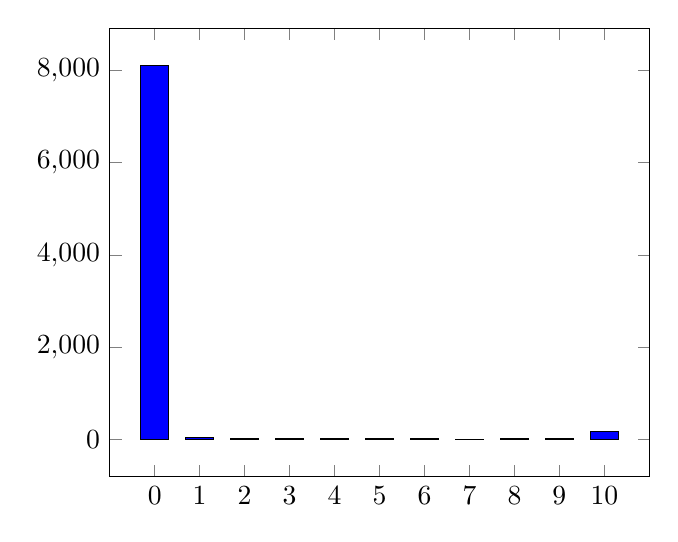
\begin{tikzpicture}
\begin{axis}[xtick=data]
\addplot[ybar,fill=blue] coordinates {
(0,8106)
(1,40)
(2,22)
(3,17)
(4,11)
(5,13)
(6,13)
(7,7)
(8,13)
(9,10)
(10,174)
};
\end{axis}
\end{tikzpicture}

\caption{{\bf Bimodal distribution of two-way classifiers}}
\end{center}
\label{Figure_1}
\end{figure}


\medskip\noindent The distribution is sharply bimodal, with only 1.7\% of the
data in the middle, but this is to be expected from votes obtained from
classifiers built to detect the same classes. The classifiers, both
individually and collectively, identify a vast class of digitally dead
languages that subsume over 96\% of our entire data. 

We emphasize that this massive die-off is not some future event that could, by
some clever policies, be avoided or significantly mitigated -- the deed is
already done. We have identified a small group of about 170 languages (2\%)
that are ascending, or have already ascended, to the digital realm,
and perhaps there is some hope for the 140 `borderline' languages (1.7\%) in
the middle, a matter we shall discuss in the concluding section. 

\section*{Discussion}

While the sheer magnitude of the failure to ascend is clear from the preceding, it
would make no sense to declare some borderline language vital or {\color{black} still}
based on the result of any single classifier. Such individual judgment could
only be made based on specific facts about the language in question, facts
that need not be encoded in our dataset, and we see many examples of languages
whose digital future is unwritten. That said, we can still demonstrate that
the overall picture is remarkably robust under changes to the details of our
method. 

Because vital languages already have their survival assured, while heritage
preservation is still very much an uphill battle, we looked more closely at
3-way classifiers that distinguishes heritage from still, but not thriving
from vital. The best S-H-VT models discussed so far utilize 6-8 features,
and have a precision of 97.1-100\% based on 10-fold crossvalidation. To test
robustness we randomized seed selection in the following manner.

We run two hundred paired experiments. For the first hundred $S_2$ seeds we
randomly take 75 languages from the group of 6,541 languages with no
detectable live online presence, and another 75 for $S_3.$ For $V_2$ we take
40 from the 83 unambiguously vital languages collected in $V_0$, and use
another 40 for $V_3$. The $T_2$ and $T_3$ seeds are defined by taking the top
16 software support and the top 16 wikipedia languages -- these seeds overlap
in 13. The $H_2$ and $H_3$ seeds will overlap completely, as we use the union
of our earlier $H_0$ and $H_1$. Thus, each classifier pair is built on 148
languages, of which only 20.3\%, the heritage class and the bulk of the
thriving, are shared across the pair. We chose this method to avoid any
appearance of bias, since the heritage status of the languages we listed above
with $H_0$ and $H_1$ is hardly debatable, while many languages like Scots or
Yiddish that would fall in the heritage class based on the vote of the first
stage classifiers will still have strongly identified users who will, perhaps,
dispute the classification the models provide.

When we look at the resulting S-H-VT-2 and S-H-VT-3 classifiers at 8
dimensions, there are small differences not just in the numerical parameters,
but also in the dimensions selected: for example, some classifiers consider it
relevant whether the language has an incubator wikipedia, while others ignore
this factor and rely on the log number of L2 speakers instead. Nor are the
classifiers perfect: internal testing (10-fold crossvalidation) shows
accuracies of 95.8\% on the average, with 2.1\% variance. But when all is said
and done, all these classifiers are highly correlated: binary classifiers
built on the same pairs of seeds correlate with each other to 0.889$\pm$0.04.
As a further check, in another hundred paired experiments we eliminated
overlap completely. The resulting classifiers have very small heritage and 
thriving seeds, but the paired classifiers still correlate 0.823$\pm$0.088,
remarkably high considering that these pairs don't share any training examples
between them.

The first 200 classifiers, using 80\% disjoint seeds (with the commonalities
restricted to the unambiguous thriving and heritage cases as described above)
estimate the digitally dead class to contain 8,049$\pm$36 languages. The
second 200, using completely disjoint seeds, shifts this number to
8,008$\pm$69.  These classifiers, having been built on smaller seeds, are less
reliable, but the overall picture is the same. No matter how we look at it, we
have over 8,000 digitally dead languages, a quarter more than the 6,541 with
no detectable online presence that we started out with.  We estimate the size
of the heritage subclass of the dead class by the same method to be
289$\pm$308, and the size of the digitally vital class (including the
thriving languages) as 377$\pm$36, and will add one sigma to speak, rather
optimistically, about 420 survivors.  Altogether we estimate the rate of
extinction to be 95.5\%, with an uncertainty of about 0.4\%.

For the following Figure~2 we selected a typical S-H-VT classifier pair, which
has Spearman (rank) correlation 0.853 (Pearson correlation on a 0-1-2 scale
would be 0.906). Whenever the two classifiers agreed, we used this result.  We
treat the 162 languages on which these disagree as members of an ad hoc `B'
(borderline) class, and break out the original 16 thriving languages from the
VT (ascended) class, so that we can report results separately on vital and
thriving. We plot only wikipedia (including incubator) languages. The $x$ axis
(log scaled) gives the number of speakers (plus one, so as not to make dead
languages fall off the scale). The $y$ axis, also log scaled, shows the
adjusted wikipedia size. The diameter of the dot is proportional to the real
ratio defined at the end of the Methods section.

\newpage
%\begin{figure}
%\vspace*{-8mm}\hspace*{-20mm}\includegraphics[width=20cm]{Stat/wpscatter3}

%\caption{
%{\bf Main parameters of wikipedia languages}
%}
%\label{Figure_2}
%\end{figure}
Adjusted wikipedia size plotted against number of speakers, log-log scales.
Dot size shows real ratio, color shows status: {\bf T}hriving dark green; {\bf
  V}ital light green; {\bf H}eritage blue; {\bf S}till black; {\bf B}orderline
red. See main text for definitions, Data Supplement S1 for underlying data.




\medskip
The 16 thriving languages, plotted in dark green on Fig. 2, have their
digital future assured, at least on a hundred year scale -- clearly wherever
humanity goes these languages will go with them. The average number of native
speakers in this group is 174.4m, the real ratio is 0.34$\pm$0.10, and the
average adjusted wikipedia size is 1.63g chars. Note that one of the six
languages that receive the best (0) EGIDS rating, Arabic, while clearly
digitally vital, has not reached thriving status yet, since Apple did not
offer OS-level support at the time we collected the data and the Arabic
wikipedia is still not in the top twenty. 

Of the 252 additional languages classified vital, plotted in light green, only
the original 83 forming the $V_0$ and $V_1$ seeds have unambiguously vigorous
language use, manifested in a significant digital community that generates
millions of words of online material per year -- the rest are largely
borderline. Experience with the individual cases suggests that no more than
150 of these languages are actually vital but, in keeping with the
conservative methodology outlined at the beginning, we are prepared to
overestimate the vitality of the rest.  The average number of native speakers
in this group is 15.9m, the real ratio is 0.22$\pm$0.18, and the average
adjusted wikipedia size is 32.5m chars.  While there is work to be done to
make these languages truly thrive in the digital realm (for example, Hungarian
is supported by Microsoft Word on the PC, but not on the Mac), we have little
doubt that the rising tide of digitization will, in the next hundred years,
carry at least half of them, hopefully even more. This group contains about
two thirds (66\%) of the EGIDS 1 languages; less than half (46\%) of EGIDS 2;
13\% of EGIDS 3; 8\% of EGIDS 4; 2\% of EGIDS 5; and less than 1\% of all
higher classes, for an average EGIDS of 3.3.

%t_egids	0.69	0.46	1.00	
%v_egids	3.29	1.98	3.00
%b_egids	5.73	1.90	6.00
%h_egids	7.83	0.93	7.70	
%s_egids	6.04	1.51	6.00
	

We emphasize that the 162 borderline languages, plotted in red, are not
classifed `borderline' but rather indicate the uncertainties inherent in the
classification. The statistical summaries in Table~2 include these as well for
the sake of completeness, but are not explained here, as these pertain to the
margins rather than to true class averages. 

There are 51 heritage languages with Wikipedias, plotted in blue.  Most of
these wikipedias are grandfathered, because they were established before the
current policy of banning dead languages was established, and it is likely
that other heritage projects such as Classical Greek will eventually find a
home on Wikia (as opposed to {\tt wikipedia.org}). The average number of
speakers is 8,787 (because several languages like Breton and Proven\,cal are
listed with significant numbers of L1 speakers in the Ethnologue), the real
ratio is 0.10$\pm$0.12 (we consider any real ratio above .1 reasonable), and
the adjusted wikipedia size is 2.25m chars. The large EGIDS average, 7.83, is
quite reflective of their heritage status. Typical examples (as found by the
classifiers, as opposed to the manually selected seeds listed in Methods)
include Cree (cre), Dalmatian (dlm), Middle Dutch (dum), Ido (ido), Gothic
(got), Old Norse (non), Pipil (ppl), Old Prussian (prg), Romagnol (rgn), and
Samogitian (sgs).

There are 307 still languages, plotted in black, where no digital
natives can be raised. The average number of speakers is 0.7m, still quite
sizeable, but the wikipedias are mostly incubators, essentially empty after
adjustment. A typical example is Kanuri (kau), with main dialects Tumari
(krt), Manga (kby), and Beriberi (knc), with EGIDS status 6a, 5, and 3
respectively. With vigorous language use, radio and TV broadcasts in the
language, and a total of 3.76m speakers, the language, at least the Central
(Beriberi) dialect, is not on anybody's radar as endangered -- to the
contrary, there are only 337 languages with EGIDS 3 or better. Yet the
wikipedia was closed for lack of native language content and community, and
the Cr\'ubad\'an crawl listing three documents for less than 5,000 words
total. The average EGIDS rating is 6.04, and the majority of the world's
languages are within one sigma of this value, consistent with our assessment
that the majority of the world's languages are digitally still.

%t_wp_siz 1630.90m	2152.20m	877.39m
%v_wp_size	32.52m	90.37m	0.74m
%b_wp_size	2.17m	14.21m	2926.50
%h_wp_size	2.25m	9.55m	17717.00	
%s_wp_size	31.30	458.72	1.00	
%t_l1	174.35m	288.11m	67.448461m	
%v_l1	15.86m	60.91m	3.12m	
%b_l1	1.39m	4.24m	101001	
%h_l1	8786.63	36177.3	1.00	
%s_l1	694512	2.46m	30000.10	
\begin{table}
\begin{center}
\caption{
\bf{Summary characteristics of languages by class}}
\begin{tabular}{|l|l|l|r|r|r|r|r|r|}
\hline
class &  lang & r/t &  $\overline{WP}$ & $\widetilde{WP}$ & $\overline{L1}$ & $\widetilde{L1}$ & $\mu_E$ & $\sigma_E$\\
\hline
{\bf T} & 16 & 0.336 & 1630.9 & 877.4& 174.4m & 67.4m & 0.69 & 0.46\\
{\bf V} & 252 & 0.225 & 32.5 & 0.74  & 15.9m & 3.1m & 3.29 & 1.98\\
{\bf B} & 162 & 0.148 & 2.17 & 0.003 & 1.39m & 0.1m & 5.73 & 1.90\\
{\bf H} & 51 & 0.144  & 2.25 & 0.018 & 8.79k & 0 & 7.83 & 0.93\\
{\bf S} & 307 & 0.003 & 0.00003 & 0 & 695k & 30k & 6.04 & 1.51\\
\hline
\end{tabular}
\begin{flushleft} Class: {\bf T}hriving, {\bf V}ital,   {\bf B}orderline,
  {\bf H}eritage, {\bf S}till.  lang: number of languages in
  class. r/t:~ratio of real to total number of pages. $\overline{WP}$: average
  adjusted Wikipedia size (millions of characters,
  entropy adjusted). $\widetilde{WP}$: median adjusted Wikipedia size
  (millions of characters,   entropy-adjusted). $\overline{L1}$:
  average number of native speakers. $\widetilde{L1}$:
  median number of native speakers. 
  $\mu_E$: average EGIDS rating.
  $\sigma_E$ variance of EGIDS rating. 
\end{flushleft}
\label{tab:label}
\end{center}
 \end{table}

\section*{Conclusions}

{\color{black} We have machine classified the world's languages as digitally
  ascending (including all vital, thriving, and borderline cases) or not, and
  concluded, optimistically, that the former class is {\it at best} 5\% of the
  latter. Broken down to individual languages and language groups t}he
situation is quite complex and does not lend itself to a straightforward
summary.  In our {\color{black} subjective} estimate, no more than a third of the
incubator languages will make the transition to the digital age. As the
example of the erstwhile Klingon wikipedia (now hosted on Wikia) shows, a
group of enthusiasts can do wonders, but it cannot create a genuine
community. The wikipedia language policy, {\tt
  https://meta.wikimedia.org/wiki/Language\_proposal\_policy}, demanding that
``at least five active users must edit that language regularly before a test
project will be considered successful'' can hardly be more lenient, but the
actual bar is much higher. Wikipedia is a good place for digitally-minded
speakers to congregate, but the natural outcome of these efforts is a heritage
project, not a live community.

A community of wikipedia editors that work together to anchor to the web the
culture carried by the language is a necessary but insufficient condition of
true survival. By definition, digital ascent requires use in a broad
variety of digital contexts. This is not to deny the value of heritage
preservation, for the importance of such projects can hardly be overstated,
but language survival in the digital age is essentially closed off to local
language varieties whose speakers have at the time of the Industrial
Revolution already ceded both prestige and core areas of functionality to the
leading standard koin\'es, the varieties we call, without qualification,
French, German, and Italian today. 

A typical example is Piedmontese, still spoken by some 2-3m people in the
Torino region, and even recognized as having official status by the regional
administration of Piedmont, but without any significant digital presence.
More closed communities perhaps have a better chance: Faroese, with less than
50k speakers, but with a high quality wikipedia, could be an example.  There
are glimmers of hope, for example \cite{flanderstoday:12-06-12} reported
40,000 downloads for a smartphone app to learn West Flemish dialect words and
expressions, but on the whole, the chances of digital survival for those
languages that participate in widespread bilingualism with a thriving
alternative, in particular the chances of any minority language of the British
Isles, are rather slim. 

In rare cases, such as that of Kurdish, we may see the emergence of a digital
koin\'e in a situation where today separate Northern (Kurmanji), Central
(Sorani), and Southern (Kermanshahi) versions are maintained (the latter as an
incubator). But there is no royal road to the digital age. {\color{black} While
  our study is synchronic only, the diachronic path to literacy and digital
  literacy is well understood: it takes a Caxton, or at any rate a significant publishing
  infrastructure, to enforce a standard, and it takes many years of formal
  education and}
a concentrated effort on the part of the community to train computational
linguists who can develop the necessary tools, from transliterators (such as
already powering the Chinese wikipedia) to spellcheckers and machine
translation for their language. Perhaps the most remarkable example of this is
Basque, which enjoys the benefits of a far-sighted EU language policy, but
such success stories are hardly, if at all, relevant to economically more
blighted regions with greater language diversity. 

The machine translation services offered by Google are an increasingly
important driver of cross-language communication. As expected, the first
several releases stayed entirely in the thriving zone, and to this day all
language pairs are across vital and thriving languages, with the exception of
French -- Haitian Creole.  Were it not for the special attention DARPA, one of
the main sponsors of machine translation, devoted to Haitian Creole, it is
dubious we would have any MT aimed at this language. There is no reason
whatsoever to suppose the Haitian government would have, or even could have,
sponsored a similar effort \cite{Spice:2010}.  Be it as it may, Google
Translate for any language pair currently likes to have gigaword corpora in
the source and target languages and about a million words of parallel
text. For vital languages this is not a hard barrier to cross. We can
generally put together a gigaword corpus just by crawling the web, and the
standardly translated texts form a solid basis for putting together a parallel
corpus \cite{Varga:2007}.
%(Varga et al 2007). 
But for borderline languages this is a real problem, because online material
is so thinly spread over the web that we need techniques specifically designed
to find it \cite{Scannell:2007}, and even these techniques yield only a drop
in the bucket: instead of the gigaword monolingual corpora that we would need, the
average language has only a few thousand words in the Cr\'ubad\'an crawl. To
make matters worse, the results of this crawl are not available to the public
for fear of copyright infringement, yet in the digital age what cannot be
downloaded does not exist.

The {\color{black} digital} situation is far worse than the consensus figure of
2,500 to 3,000 endangered languages would suggest. Even the most pessimistic
survey \cite{Krauss:1992}
% (Krauss 1992) 
assumed that as many as 600 languages, 10\% of the population, were
safe, but reports from the field increasingly contradict this. For British 
Columbia, \cite{Poser:pc} writes:

\begin{quote}
Here in BC, for example, the prospect of the survival of the native languages
is nil for all of the languages other than Slave and Cree, which are somewhat
more viable because they are still being learned by children in a few remote
communities outside of BC. The native-language-as-second-language programs are
so bad that I have NEVER encountered a child who has acquired any sort of
functional command (and I don't mean fluency - I mean even simple
conversational ability or the ability to read and understand a fairly simple
paragraph or non-ritual bit of conversation) through such a program. I have
said this publicly on several occasions, at meetings of native language
teachers and so forth, and have never been contradicted. Even if these
programs were greatly improved, we know, from e.g. the results of French
instruction, to which oodles of resources are devoted, that we could not
expect to produce speakers sufficiently fluent to marry each other, make
babies, and bring them up speaking the languages. It is perfectly clear that
the only hope of revitalizing these languages is true immersion, but there are
only two such programs in the province and there is little prospect of any
more.  The upshot is that the only reasonable policy is: (a) to document the
languages thoroughly, both for scientific purposes and in the hope that
perhaps, at some future time, conditions will have changed and if the
communities are still interested, they can perhaps be revived then; (b) to
focus school programs on the written language as vehicle of culture, like
Latin, Hebrew, Sanskrit, etc. and on language appreciation. Nonetheless, there
is no systematic program of documentation and instructional efforts are aimed
almost entirely at conversation.
\end{quote}

\noindent
Cree, with a population of 117,400 (2006), actually has a wikipedia at {\tt
  http://cr.wikipedia.org} but the real ratio is only 0.02, suggestive of a
hobbyist project rather than a true community, an impression further supported
by the fact that the Cree wikipedia has gathered less than 60 articles in the
past six years. Slave (3,500 speakers in 2006) is not even in the incubator
stage. This is to be compared to the over 30 languages listed by the Summer
Institute of Linguistics for BC.  In reality, there are currently less than
250 digitally ascending languages worldwide, and {\color{black} about half of
  the borderline cases are like Moroccan Arabic (ary), low prestige spoken
  dialects of major languages whose signs of vitality really originate with
  the high prestige acrolect. This suggests that in the long run no more} than
a third of the borderline cases will become vital. One group of languages that
is particularly hard hit are the 120+ signed languages currently in use. Aside
from American Sign Language, which is slowly but steadily acquiring digital
dictionary data and search algorithms \cite{Thangali:2011},
%(Thangali et al 2011), 
it is perhaps the emerging International Sign \cite{Hiddinga:2011}
%(Hiddinga and Crasborn 2011) 
that has the best chances of survival. 

There could be another 20 spoken languages still in the wikipedia incubator
stage or even before that stage that may make it, but every one of these will
be an uphill struggle.  Of the 7,000 languages still alive, perhaps 2,500 will
survive, in the classical sense, for another century. With only 250 digital
survivors, all others must inevitably drift towards digital heritage status
(Nynorsk) or digital extinction (Mandinka). This makes language preservation
projects such as {\tt http://www.endangeredlanguages.com} even more
important. To quote from \cite{UN_biodiv:2004}:

\begin{quote}
Each language reflects a unique world-view and culture complex, mirroring the
manner in which a speech community has resolved its problems in dealing with
the world, and has formulated its thinking, its system of philosophy and
understanding of the world around it.  In this, each language is the means of
expression of the intangible cultural heritage of people, and it remains a
reflection of this culture for some time even after the culture which
underlies it decays and crumbles, often under the impact of an intrusive,
powerful, usually metropolitan, different culture.  However, with the death
and disappearance of such a language, an irreplaceable unit in our knowledge
and understanding of human thought and world-view is lost forever.
\end{quote}

\noindent
Unfortunately, at a practical level heritage projects (including wikipedia
incubators) are haphazard, with no systematic programs of
documentation. Resources are often squandered, both in the EU and outside, on
feel-good revitalization efforts that make no sense in light of the
preexisting functional loss and economic incentives that work against language
diversity \cite{Ginsburgh:2011}.
%(Ginsburgh and Weber 2011).  

Evidently, what we are witnessing is not just a massive die-off of the
world's languages, it is the final act of the Neolithic Revolution, with the
urban agriculturalists moving on to a different, digital plane of existence,
leaving the hunter-gatherers and nomad pastoralists behind. As an example,
consider Komi, with two wikipedias corresponding to the two main varieties
(Permyak, 94,000 speakers and Zyrian, 293,000 speakers), both with alarmingly
low ($< 0.02$) real ratios. Given that both varieties have several dialects,
some already extinct and some clearly {\color{black} still}, the best hope is for a koin\'e to
emerge around the dialect of the main city, Syktyvkar. Once the orthography is
standardized, the university (where the main language of education is Russian)
can in principle turn out computational linguists ready to create a
spellchecker, an essential first step toward digital literacy \cite{Proszeky:2005}.
% (Pr\'osz\'eky and Nov\'ak 2005). 
But the results will benefit the koin\'e speakers, and the
low prestige rural Zyrian dialects are likely to be left behind.

What must be kept in mind is that the scenario described for Komi is
optimistic. There are several hundred thousand speakers, still amounting to
about a quarter of the local population. There is a university. There are
strong economic incentives (oil, timber) to develop the region further. But
for the 95\% of the world's languages where one or more of these drivers are
missing, there is very little hope of crossing the digital divide.

\section*{Appendix}

Supporting information S1, also accessible at {\tt
  http://hlt.sztaki.hu/resources/dld-joined.tsv} used the latest (February
2012) Ethnologue dump, and May 2012 Wikipedia dumps except for the incubator
projects, which multiplied rapidly at the time. The incubators at Wikimedia,
OLAC, ELP, and the Cr\'ubad\'an sites were crawled in March 2013.  Software
readiness reflects MacOS 10.6.8 and Windows 7, Google Translate was assessed
December 2012. Features marked by {\bf log} are incremented by one and log
transformed before classification. Features marked by {\bf ignore} were not
used as input to the classification, they are presented only to help the
readers search for particular languages. The abbreviations here are taken
verbatim from the header of the main table.


\noindent\begin{enumerate}
\item unique\_join\_code -- SIL or Linguist List code where available.  For
  languages without clearly identifiable SIL code in ELP and Cr\'ubad\'an
  non-authoritative codes beginning with {\tt xxe} and {\tt xxx} were
  generated {\bf ignore}
\item wikiname -- the two-letter (sometimes longer) code used in Wikipedia {\bf ignore} 
\item EthLanguageStatus -- the EGIDS status of the language according to the
  Ethnologue. Values 6b and 8b were replaced by 6.5 and 8.5 so as to keep the
  other values of the scale intact. The Ethnologue is fairly complete: based on
  lack of overlap with other language lists we estimate its coverage on
  non-extinct non-artificial languages to be well above 90\%. At this stage,
  non-threatened languages are highly unlikely to be added, so for such
  languages we supplied an EGIDS value of 7.7, the weighted average of the
  threatened classes
\item L1 -- number of people speaking the language natively (L1
  speakers) {\bf log}
\item L2 -- number of people speaking the language as second language (L2
  speakers) {\bf log}
\item MACinput -- input-level support by Apple
\item MACsupp -- OS-level support in MacOS 10.6.8
\item MSifpack -- input-level support by Microsoft
\item MSpack -- OS-level support in Windows 7.
\item TLDs -- whether a national level Top Level Domain (not {\tt .com, .org,
  .edu}) appeared in the top three domains that the crawl found language data
  in. Potentially a proxy for national-level organization in cyberspace 
\item WPincubatornew -- whether Wikipedia had an incubator for the language in
  March 2013
\item WPsizeinchars -- raw (unadjusted) character count of wikipedia {\bf log}
\item adjustedWPsize -- character count of `real' wikipedia pages, normalized
  for character entropy {\bf log}
\item articles -- number of articles in wikipedia {\bf log}
\item realtotalratio -- proportion r/t of `real' wikipedia pages
\item avggoodpagelength -- average length of `real' wikipedia pages {\bf log}
\item cru1Characters -- number of characters found by the first Cr\'ubad\'an
  crawl {\bf log}
\item cru1Docs -- number of documents found by the first Cr\'ubad\'an crawl
  {\bf log}
\item cru1FLOSSSplChk -- whether a FLOSS spellchecker exists according to the 
  first Cr\'ubad\'an summary
\item cru1UDHR -- whether a translation of the Universal Declaration of Human
  rights exists according to the first Cr\'ubad\'an summary
\item cru1WT -- whether an online Bible 
  exists at {\tt watchtower.org} according to the first Cr\'ubad\'an summary
\item cru1Words -- number of words found by the first Cr\'ubad\'an crawl {\bf log}
\item cru2Characters {\bf log}, cru2Docs {\bf log}, cru2FLOSSSplChk,
  cru2MSinput, cru2UDHR, cru2WT, cru2Words {\bf log} -- same as above, except
  data is taken from the second Cr\'ubad\'an crawl.
\item endclass -- classification according to the Endangered Languages
  Project: at risk: 4; vulnerable: 5; threatened: 6; endangered/unknown: 7; 
critically endangered: 8; severely endangered: 9. Since the project aims at 
completeness, languages it excludes are assigned to class 2
\item hunspellcoverage -- the percentage coverage Hunspell has on the
  wikipedia dump
\item hunspellstatus -- whether a HunSpell spellchecker exists for the language
\item inomni -- whether the language is written in a script listed in Omniglot
\item laPrimarytextsOnline -- the number of OLAC primary texts online {\bf log}
\item seedstatus -- training labels manually set to C, V, H, or M for
  languages in the respective seeds
\item cru2Classification -- The more elaborate linguistic classification
  listed in Cr\'ubad\'an {\bf ignore} 
\item PrintName -- standardized English language name {\bf ignore} 
\item LanguageLocal -- the local name of the language {\bf ignore} 
\item cru2NameNative -- the local name of the language according to
  Cr\'ubad\'an {\bf ignore} 
\item sample\_result -- the result of voting together two paired classifiers
     {\bf ignore} 

\end{enumerate}



INSERT PLOS LINK TO SUPPLEMENTARY DATA ABOUT HERE


\section*{Acknowledgments}

The author was greatly helped in the data gathering by the Human Language
Technology group at the Hungarian Academy of Sciences Computer and Automation
Research Institute, in particular by Attila Zs\'eder who unified the data
coming from many sources, and Katalin Pajkossy who ran the maxent.  We thank
Tam\'as V\'aradi (Hungarian Academy of Sciences), Hans Uszkoreit (Saarland
University at Saarbr\"ucken) and Georg Rehm (DFKI Berlin) for the opportunity
to present an earlier version of this material at the Multilingual Europe
Technology Alliance (META) Forum 2012 in Brussels. Comments by Onno Crasborn
(Radboud University Nijmegen) and Bill Poser (Yinka Dene Language Institute)
have led to significant improvements. {\color{black} Comments by the Editor and
  anonymous referees have led to very significant improvements.}  We thank
Judit \'Acs, M\'arton Makrai, G\'abor Recski, (HAS Computer and Automation
Research Institute) and Taha Yasseri (Oxford) for research assistance.  Work
supported by OTKA grant \#82333.

%\section*{References}
% The bibtex filename
%\bibliography{template}

\bibliographystyle{plos2009}
\bibliography{ml}

\end{document}
\newpage

\section*{Figures}

\newpage 



\end{document}


\keywords{language death, cultural heritage, wikipedia}




\cite{Thangali:2011} 
